\documentclass[12pt, paper=a4]{article}
\usepackage[utf8]{inputenc}
\usepackage[german]{babel}
\usepackage{mathrsfs}
\usepackage{amsmath}
\usepackage{amssymb}
\usepackage{listings}
\usepackage{graphicx}
\usepackage{fancyhdr}

\setlength{\parindent}{0pt}

\author{Mareike Göttsch, 6695217, Gruppe 2\\Paul Hölzen, 6673477, Gruppe 1\\Sven Schmidt, 6217064, Gruppe 1}

\title{FGI 2 Hausaufgaben 5}

\rhead{M. Göttsch, G-2; P. Hölzen, G-1; S. Schmidt, G-1}
\pagestyle{fancy}
\begin{document}
\maketitle

\section*{Aufgabe 5.3}
\subsection*{1.}
\subsubsection*{(a)}
\begin{align*}
f &= \mathbf{AF}(\neg( orbit \Rightarrow away)) \land \neg\mathbf{AG}( \mathbf{E}( orbit\mathbf{U}warp)) \\ &=  \mathbf{AF}(\neg(\neg orbit\lor away))\land\neg\neg \mathbf{EF}(\neg \mathbf{E}(orbit\mathbf{U}warp)) \\ &= \neg \mathbf{EG}(\neg orbit\lor away)\land \mathbf{E}(True\mathbf{U}(\neg \mathbf{E}(orbit\mathbf{U}warp)))
\end{align*}
\subsubsection*{(b)}
\begin{align*}
g_{1} &= \mathbf{AGEF}(warp) \\ &= \neg \mathbf{EF}(\neg\mathbf{EF}(warp)) \\ &= \neg\mathbf{E}(True\mathbf{U}(\neg\mathbf{E}(True\mathbf{U}warp)))
\end{align*}
\begin{align*}
g_{2} &= \mathbf{EFAG}(warp) \\ &=\mathbf{E}(True\mathbf{U}(\neg \mathbf{EF}(\neg warp))) \\
&= \mathbf{E}(True\mathbf{U}(\neg \mathbf{E}(True\mathbf{U}\neg warp)))
\end{align*}

\subsection*{2.}
Eine natürlich-sprachliche Beschreibung für $f$ wäre:
\begin{quote}
	Es gibt keinen Pfad auf dem immer 'away' oder nicht 'orbit' gilt und es gibt einen Pfad, auf dem irgendwann kein Pfad existiert, auf welchem solange 'orbit' gültig ist bis 'warp' gilt.
\end{quote}
Eine natürlich-sprachliche Beschreibung für $g_{1}$ wäre:
\begin{quote}
	Auf allen Pfaden gibt es immer einen Pfad auf dem irgendwann 'warp' gilt.
\end{quote}
Eine natürlich-sprachliche Beschreibung für $g_{2}$ wäre:
\begin{quote}
	Es gibt einen Pfad auf dem irgendwann auf allen Pfaden immer 'warp' gilt.
\end{quote}

\subsection*{3.}
\begin{align*}
Sat(f) &= Sat(\neg \mathbf{EG}(\neg orbit\lor away)\land \mathbf{E}(True\mathbf{U}(\neg \mathbf{E}(orbit\mathbf{U}warp)))) \\ &= Sat(\neg \mathbf{EG}(\neg orbit\lor away)) \cap Sat(\mathbf{E}(True\mathbf{U}(\neg \mathbf{E}(orbit\mathbf{U}warp))))
\end{align*}
Es gilt $Sat(\neg orbit)=\{2,3,4\}$ und $Sat(away)=\{1\}$.\\
Daraus folgt $Sat(\neg orbit \lor away)=\{2,3,4\} \cup \{1\} = \{1,2,3,4\}$.\\
Da $SZK_{1}=\{3\}$ und $SZK_{2}= \{2,3,4\}$ die einzigen SZKs von $\neg orbit \lor away$ sind gilt: $Sat( \mathbf{EG}(\neg orbit\lor away))=T=\{2,3,4\}$
Daraus folgt dann wiederum: \[Sat(\neg \mathbf{EG}(\neg orbit\lor away))=\{0,1\}  \]
Für den zweiten Teil der Und-Verknüpfung gilt $Sat(warp)=\{2\}$. Daraus folgt durch schrittweises Einsetzten in Gegenrichtung:\[ Sat(\mathbf{E}(orbit\mathbf{U}warp))=\{0,1\} \]
Somit gilt $Sat(\neg \mathbf{E}(orbit\mathbf{U}warp))=\{2,3,4\}$. \\
Da diese Zustände von allen anderen Zuständen erreichbar sind folgt daraus \[Sat(\mathbf{E}(True\mathbf{U}(\neg \mathbf{E}(orbit\mathbf{U}warp))))=\{0,1,2,3,4\}  \]
Für $Sat(f)$ folgt daraus schließlich:\[ Sat(f)= \{0,1\} \cap \{0,1,2,3,4\} = \{0,1\} \]
\\

Für $g_{1}$ gilt, da $Sat(warp)=\{2\}$ und $s_{2}$ von allen Zuständen erreichbar ist, dass $Sat(\mathbf{E}(True\mathbf{U}warp))=\{0,1,2,3,4\}$.\\
Demnach ist $Sat(\neg\mathbf{E}(True\mathbf{U}warp))=\emptyset$ woraus wiederum folgt, dass \[Sat(\mathbf{E}(True\mathbf{U}(\neg\mathbf{E}(True\mathbf{U}warp))))=\emptyset\]
Es gilt daher für $Sat(g_{1})$:\[Sat(g_{1})=Sat(\neg\mathbf{E}(True\mathbf{U}(\neg\mathbf{E}(True\mathbf{U}warp))))=\{0,1,2,3,4\}\]
\\
Für $g_{2}$ gilt entsprechend:
\begin{align*}
&Sat(\neg warp)=\{0,1,3,4\} \Rightarrow Sat(\mathbf{E}(True\mathbf{U}\neg warp))=\{0,1,2,3,4\} \\
	\Rightarrow& Sat(\neg\mathbf{E}(True\mathbf{U}\neg warp))=\emptyset \Rightarrow Sat(\mathbf{E}(True\mathbf{U}(\neg \mathbf{E}(True\mathbf{U}\neg warp))))=\emptyset
\end{align*}
Es gilt also: \[Sat(g_{2})=Sat(\mathbf{E}(True\mathbf{U}(\neg \mathbf{E}(True\mathbf{U}\neg warp))))=\emptyset\]
\subsubsection*{4.}
Es zeigt sich, dass $g_{1}$ auf ganz M gültig ist während $g_{2}$ auf ganz M nicht gilt.
Dies ist auch nicht verwunderlich, denn bereits aus der natürlich-sprachlichen Beschreibung für $g_{1}$ und $g_{2}$ lässt sich die Gültigkeit der beiden Formeln intuitiv ableiten.

\newpage
\section*{Aufgabe 5.4}
\subsection*{1.}
Die Transitionssysteme $R_1, R_2$ und $R_3$ mit $hi, vi \in A_i$ für alle Systeme und $AP = \{closed, fetched\}$ wobei $closed$ den Zustand beschreibt, den ein Roboter hat der gerade eine Dose verschlossen hat und $fetched$ bedeutet, dass ein Roboter einen Deckel geholt hat.\\

\begin{figure}[h!]
\centering
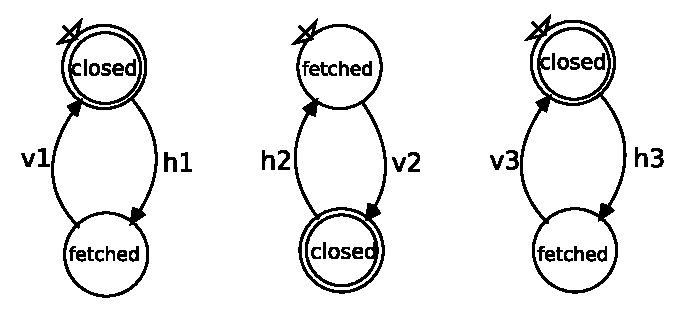
\includegraphics[scale=0.8]{r1r2r3.pdf}
\caption{Transitionssysteme $R_1, R_2$ und $R_3$}
\end{figure}

\subsection*{2.}
Das Produkttransitionssystem $R_1 \oplus R_2 \oplus R_3$ mit der Synchronisationsrelation $Sync = \{(h1, v2, h3), (v1, h2, v3)\}$.\\

\begin{figure}[h!]
\centering
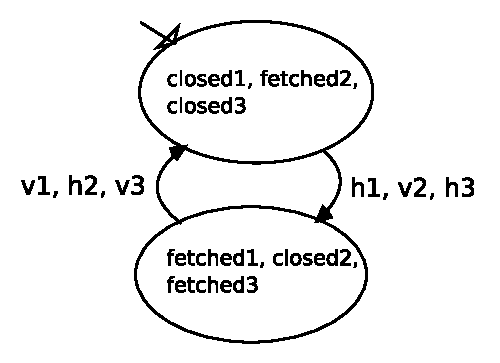
\includegraphics[scale=0.7]{r1r2r3_prod.pdf}
\caption{$R_1 \oplus R_2 \oplus R_3$}
\end{figure}

\subsection*{3.}


\end{document}
